\section{State of the art in ESD testing}
\label{sec:state-art-esd-testing}

Electronic hardware robustness is tested against electrostatic discharges using different test methods and standards.
Each method reproduces a specific discharge event \gls{esd} in laboratory conditions.
In this chapter, relevant \gls{esd} generators for this research work are detailed.

In ESD testing, a distinction is often made between so-called system-level level tests and \gls{ic} level tests.
System-level tests reproduce discharge events encountered by a system deployed in the field.
Silicon-level tests target \gls{esd} events happening during \gls{ic} manufactoring.

System-level tests involve higher voltage and current amplitudes, and are more harmful for electronic devices than \gls{ic} level tests.

\subsection{Transmission Line Pulsing (TLP)}

% History of TLP
The transmission line pulsing generator is an extremely popular tool in the \gls{esd} field.
Over the years, it was employed in a variety of applications, from characterization of devices \cite{TLPforESDProtectionCz, TLPthroubleshooting}, investigation of failures \cite{tlp-application-1, tlp-application-2} and correlation of failure levels with other generators \cite{correlation-system-level-esd-tlp}.
It is a versatile tool, that was often modified to adress larger testing conditions \cite{tlp-power} or non-rectangular pulse waveforms \cite{tlp-based-hmm, my-publi-tlp-hmm}.
The technique was invented by T. Maloney and N. Nakamura \cite{TLP}.
It is in the process of standardization as part of ANSI/ESD STM 5.5.1-2016 \cite{tlp-standard} through the effort of the ESD Association (ESDA) \cite{esda}.
It was extensively studied the PhD thesis of N. Monnereau \cite{phd-monnereau} and N. Lacrampe \cite{phd-lacrampe}.

% Concept
\gls{tlp} systems produce a fast rectangular pulse, through the discharge of a coaxial cable (Fig. \ref{tlp_concept}).
The cable is charged by a high-voltage power supply then discharged into a load by switching a relay.
The charge is performed through a high value resistor to keep the current small and avoid oscillations on the cable.
When the voltage charge of the cable reaches the desired amplitude, the relay is switched to trigger the discharge.
The coaxial cable has usually a characteristic impedance of 50\textOmega{} and a length of 10 metres, corresponding to a 100ns propagation delay.

\begin{figure}[!h]
  \centering
  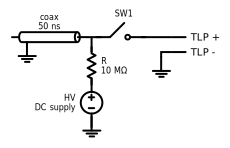
\includegraphics[width=\textwidth]{src/1/figures/tlp_concept.pdf}
  \caption{Minimal example of a \gls{tlp} system}
  \label{tlp_concept}
\end{figure}

% Characteristics of tlp systems
TLP systems constitute very well-controlled test generators where the pulse is generated inside a shielded and isolated environment.
The characteristic impedance of 50\textOmega{} can be controlled up to the load.
Those features allow for extremely clean and repeatable pulse waveforms without reflections.
The main characteristics of a TLP waveform are given in figure \ref{tlp_pulse}.
The waveform parameters are completely controlled and easily tunable.
The charging voltage is set by the high-voltage source.
The pulse width can be increased or decreased by changing the length of the coaxial cable.
The risetime can be enforced with a 50\textOmega{} matched risetime filter \cite{cao-risetime-filter, gaussian-lpf}.
Unlike most filters, they are specifically designed to work by absorption and not by reflection.
They do not pollute the system with reflected waves.

\begin{figure}[!h]
  \centering
  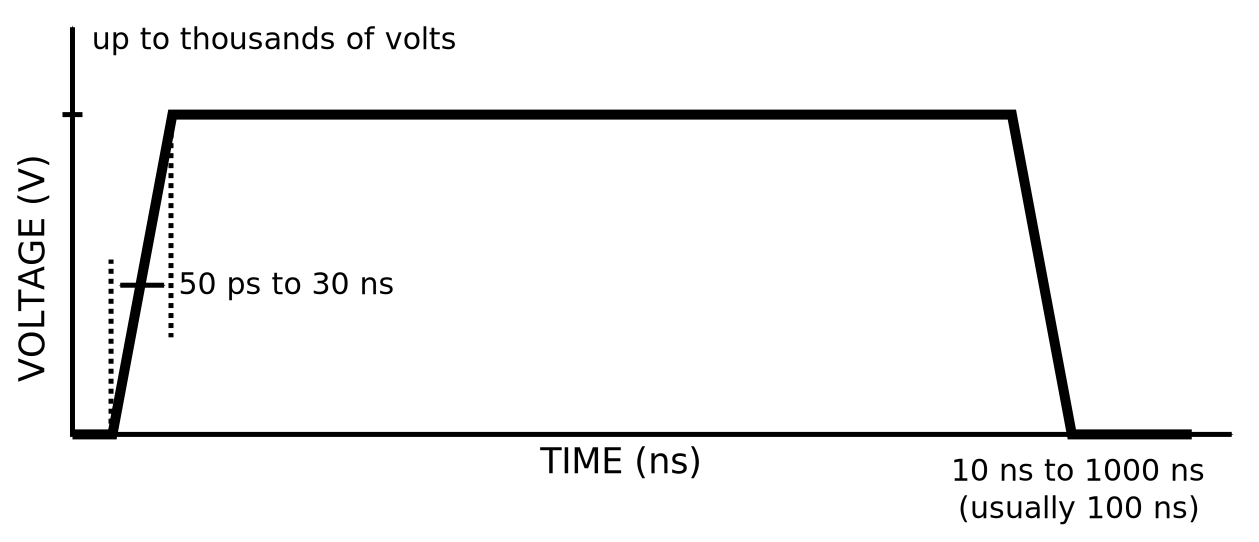
\includegraphics[width=\textwidth]{src/1/figures/tlp_pulse.pdf}
  \caption{Main characteristics of a \gls{tlp} pulse on a resistive load}
  \label{tlp_pulse}
\end{figure}

% Principle of tlp for i(v) curve extraction
%TODO: Find TLP TDR reference, and non TDR TLP ref
Time-Domain Reflectometry is a measurement technique with a wide range of applications.
Some TLP generators rely on this technique to determine electrical properties of a device by observing reflected waveforms.
In this configuration, voltage and current measured at the output of the generator are equal to voltage and current waveforms inside the load.
This is due to the superposition of the incident and reflected pulses during the discharge.
Analysis and demonstration is done in \cite{phd-monnereau}.
Other setups involve measurements directly at the load level.

% Explanation of a typical esd protection respon
Fig. \ref{fig:typical-tlp-response} provides an example of a typical waveform observed during injection on an \gls{esd} protection.
The recording is done in a time-domain reflectometry configuration, where voltage and current are measured at the ouput of the generator and not at the load.
Voltage and current waveforms usually exhibit two steps.
The first one corresponds to the impedance of the connection cable that relies the \gls{tlp} to the load (see Fig. \ref{tlp_concept}).
The second step is the response of the tested load.
By averaging each waveform during a few tens of nanosecond, the current and voltage value of the load can be sampled.
The sampled values are associated to a given charging voltage.
The process is usually very reproducible.

\begin{figure}[!h]
  \centering
  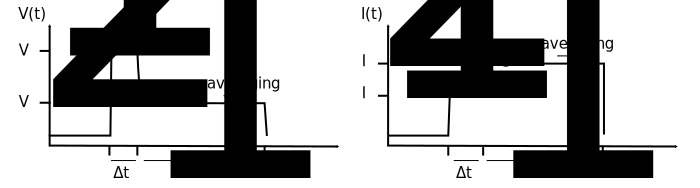
\includegraphics[width=0.3\textwidth]{src/1/figures/tlp_response.pdf}
  \caption{TLP V(t) and I(t) example}
  \label{fig:typical-tlp-response}
\end{figure}

% Main application of TLP is IV characterization
A very popular application is the extraction of a quasi-static I(V) characterization of ESD protections \cite{TLPforESDProtectionCz}.
It represents the current versus voltage response of a device, in dynamic regime.
Much higher than static I(V)
Non monotonous response

\begin{figure}[!h]
  \centering
  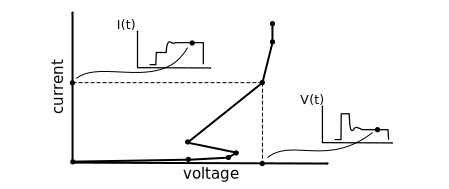
\includegraphics[width=0.3\textwidth]{src/1/figures/tlp_iv_curve.pdf}
  \caption{TLP-extracted I(V) characteristic example}
  \label{fig:iv-curve-extraction}
\end{figure}

The I(V) curve is extracted point after point, by increasing the charging voltage after each pulse (Fig. \ref{fig:iv-curve-extraction}).
Each point corresponds a voltage and current measured on the transient waveform.
Snapback waveforms are very often observed, that cannot be measured with static I(V).
%TODO: Detail more quasi-static characterization

% Another application is the characterization of the robustness
or testing the response of systems and devices against a clean and well repeatable pulse \cite{TLPthroubleshooting, LacrampeTransientImmunity}.

A popular variation of the TLP is the very fast TLP (vf-TLP), initially designed by H. Gieser \cite{vf-tlp} to reproduce gate oxyde breakdown.
It is a TLP with a shorter pulse width (10 ns).

Grund applied the principle of Time-Domain Reflectometry to vf-TLP in \cite{vf-tlp-tdr}.
With this method, it is possible analyse and calculate the impedance of all elements between the generator and the load.


\subsection{ESD Gun (IEC 61000-4-2 / ISO 10605)}

% What is the goal of this test
IEC 61000-4-2\cite{iec61000-4-2} and ISO 10605\cite{iso10605} standards define a system-level test waveform and test generator to reproduce the discharge of a human body through an electronic device.
This test is used very extensively for the qualification of products.

\begin{figure}[!h]
  \centering
  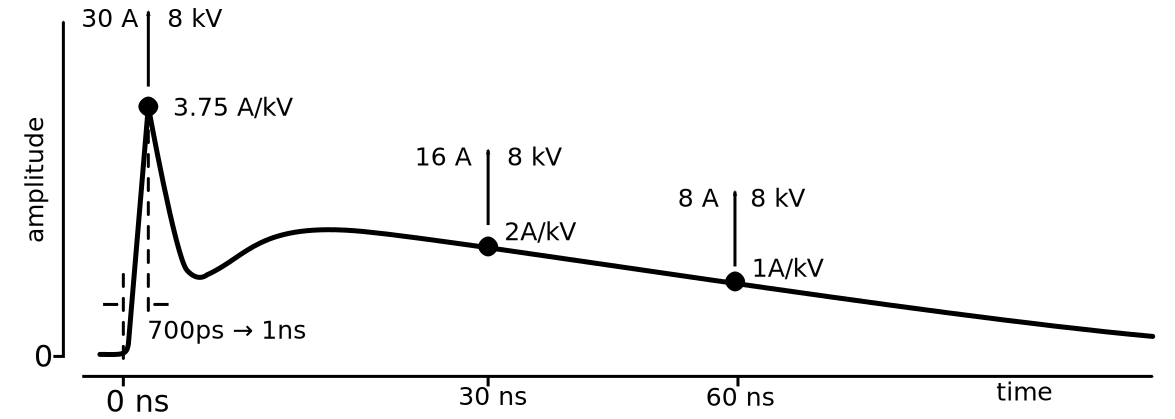
\includegraphics[width=\textwidth]{src/1/figures/iec61000-4-2_waveform.pdf}
  \caption{Main properties of an IEC 61000-4-2 pulse on a 2\textOmega\ resistive load}
  \label{iec_pulse}
\end{figure}

% How is the pulse generated
The generation of the ESD pulse is done by a resistor-capacitor discharge network.
The RC network alone though does not suffice to reproduce the waveform given in Fig. \ref{iec_pulse}.
Parasitic devices play an important part in shaping the waveform.

% Where does this standard applies
Each standard defines the construction and waveform requirements for this ESD generator, but with different fields of application.
IEC 61000-4-2\cite{iec61000-4-2} standard targets consumer electronics.
ISO 10605\cite{iso10605} standard is intented for automotive equipment.
The latter defines additional pulse waveforms to cover a wider range of ESD events (See fig \ref{iso_pulse}).

\begin{figure}[!h]
  \centering
  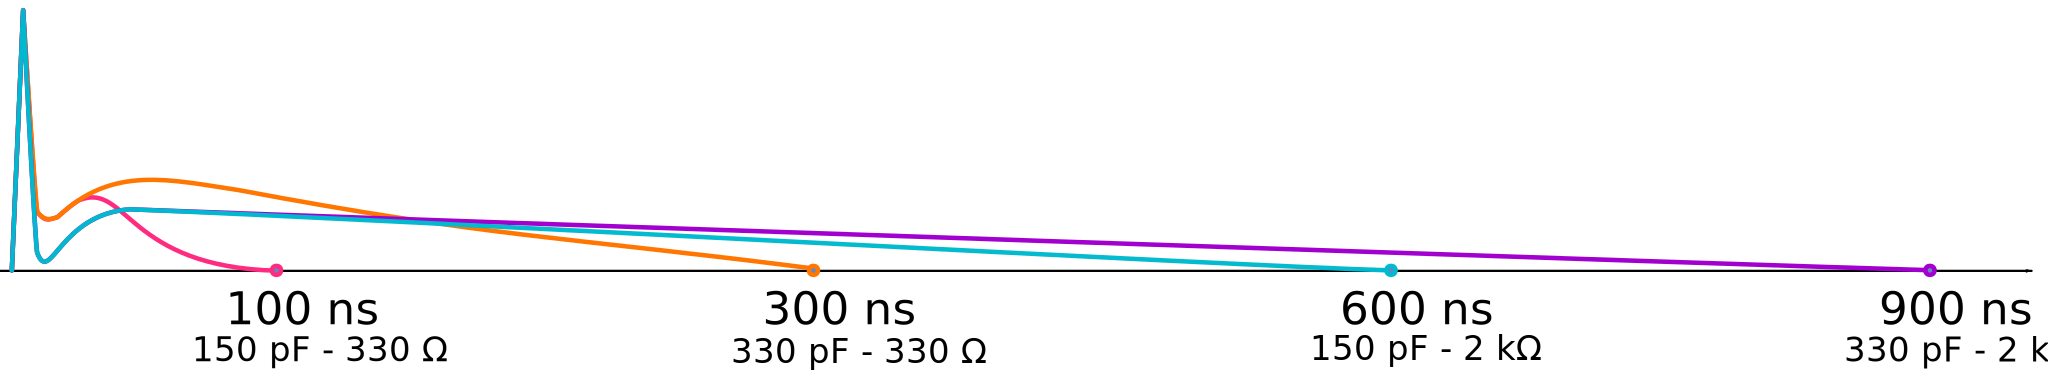
\includegraphics[width=\textwidth]{src/1/figures/iso10605_waveform.pdf}
  \caption{Waveforms defined in ISO 10605 standard on a 2\textOmega{} resistive load}
  \label{iso_pulse}
\end{figure}

%TODO: Annex F ISO 10605

\subsection{ISO 7637-2}

% Where does this standard applies
ISO 7637-2\cite{iso7637-2} is an automotive standard for testing immunity of electronic devices against transient electrical disturbances.
It is mostly targeting disturbances applied on supply lines.
This standard defines several waveforms.
Among them, pulses 2A and 3B are the closest to an electrostatic discharge.

% Pulse 2A - What is the goal of this pulse
Pulse 2A simulates the sudden disconnection of a load placed in parallel with the \gls{dut}.
In a car, it reproduces the switching of devices separated by inductive wiring harnesses.
When a load is abruptly switched off, the inductance opposes to the sudden interruption of current.
Instead of flowing through the load, the current is maintained and reported onto the \gls{dut} which can be damaged or disturbed in the process.
These events can be quite harmful with peak voltages above 50V during 50\textmu{}s.
This pulse can be an interesting testing waveform in the context of this entire document.
The characteristics of pulse 2A are given in fig. \ref{fig:iso_2a_pulse}.

\begin{figure}[!h]
  \centering
  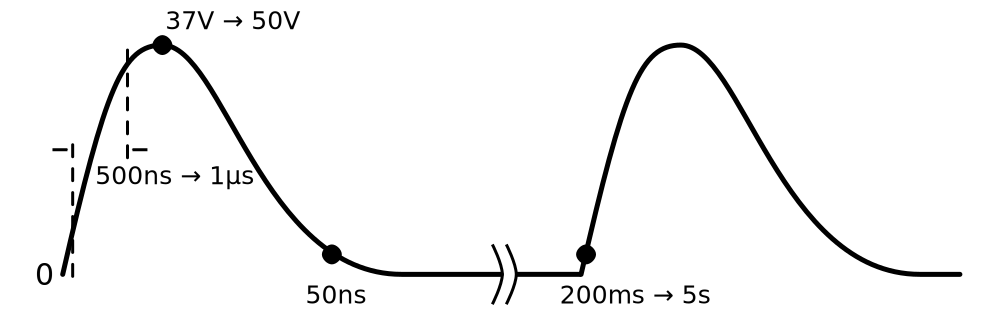
\includegraphics[width=0.7\textwidth]{src/1/figures/iso7637-2-2a.pdf}
  \caption{Waveform 2A defined in ISO 7637-2 standard on a 2\textOmega{} resistive load}
  \label{fig:iso_2a_pulse}
\end{figure}

% How is the pulse generated
ISO 7637-2 compliant stress generators are often implemented with R-C discharge networks.
It is the easiest way to produce the standardized waveform on a 2\textOmega{} resistor.
By construction, it is not the best way to reproduce the inductive behavior of the wiring harness.
However, it is a common method in the \gls{esd} field to define pulses on simple loads to make the manufacturing, testing and investigation more approachable.

% Pulse 3B - What is the goal of this pulse
Pulse 3B also simulates the result of a switching process on a wiring harness, causing negative spikes on a \gls{dut}.
Its waveform is given in fig. \ref{fig:iso_2b_pulse}.
Compared to pulse 2a, this waveform has a shorter duration and risetime and a higher amplitude.
Interestingly, it is one of the rare \gls{esd} waveforms to be defined on a 50\textOmega{} load.

\begin{figure}[!h]
  \centering
  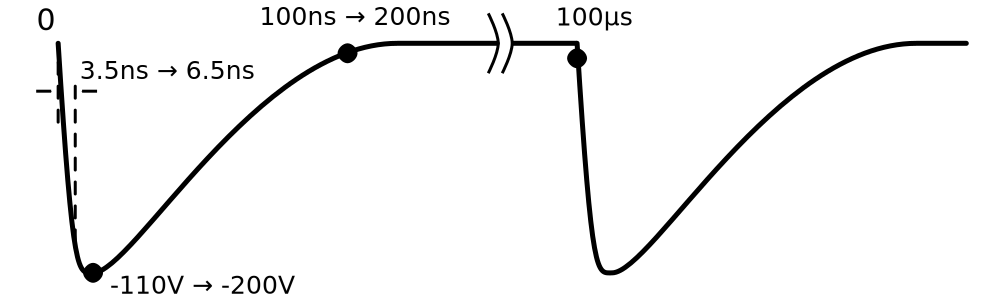
\includegraphics[width=0.7\textwidth]{src/1/figures/iso7637-2-3b.pdf}
  \caption{Waveform 3B defined in ISO 7637-2 standard on a 50\textOmega{} resistive load}
  \label{fig:iso_2b_pulse}
\end{figure}

\subsection{IEC 61000-4-4}

% Where does this standard applies - scope
The IEC 61000-4-4 standard \cite{iec61000-4-4}, also called burst test, defines a fast transient burst waveform for \gls{esd} testing.
It tests the immunity of electronic devices to repetitive fast transients on supply, signal and control ports.

% What is the pulse
The defined waveform is a double exponential pulse \ref{fig:iec_4_4_pulse} with a width of 50ns at 50\% of the peak amplitude.
It is defined for a 50\textOmega{} load, with a pulse period of 15ms and a burst period of 300ms.

\begin{figure}[!h]
  \centering
  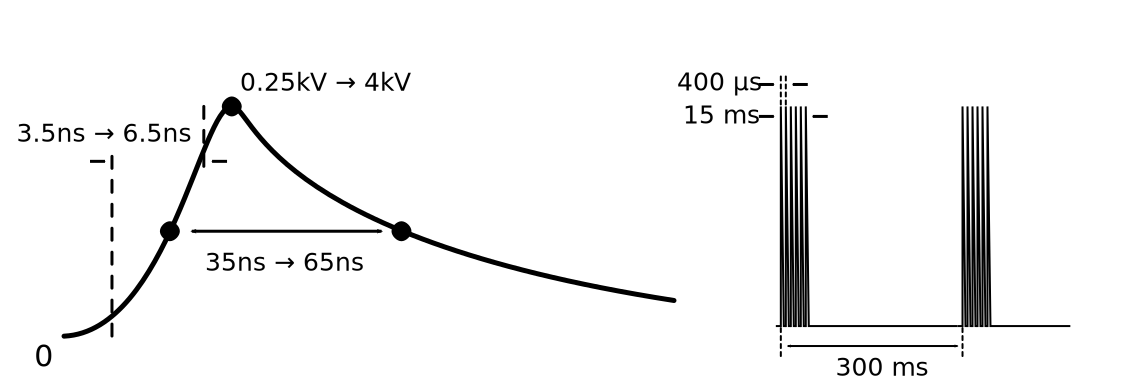
\includegraphics[width=\textwidth]{src/1/figures/iec61000-4-4_waveform.pdf}
  \caption{IEC 61000-4-4 waveform on a 50\textOmega{} resistive load}
  \label{fig:iec_4_4_pulse}
\end{figure}

% How is the pulse generated
The standard defines a circuit diagram for the generator, based on a resistor-capacitor network and spark-gap (Fig \ref{fig:iec_4_4_generator}).
The generator's output is a coaxial plug to prevent radiated emission during the discharge.

\begin{figure}[!h]
  \centering
  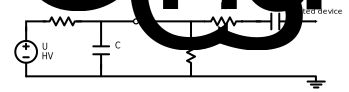
\includegraphics[width=\textwidth]{src/1/figures/iec61000-4-4_diagram.pdf}
  \caption{IEC 61000-4-4 generator circuit diagram}
  \label{fig:iec_4_4_generator}
\end{figure}

% Injection method - capacitive coupling clamp
This standard defines an injection method for powered lines called a \texit{capacitive coupling clamp} (Fig. \ref{fig:iec_4_4_clamp}).
This device is very relevant for this research work because injecting \gls{esd} onto powered devices and supplies in particular with good repeatability is rather challenging.
The device works by placing two large metallic plates in parallel, injecting the discharge on one of the plates and the wires inside a metallic tunnel connected to the other plate.

\begin{figure}[!h]
  \centering
  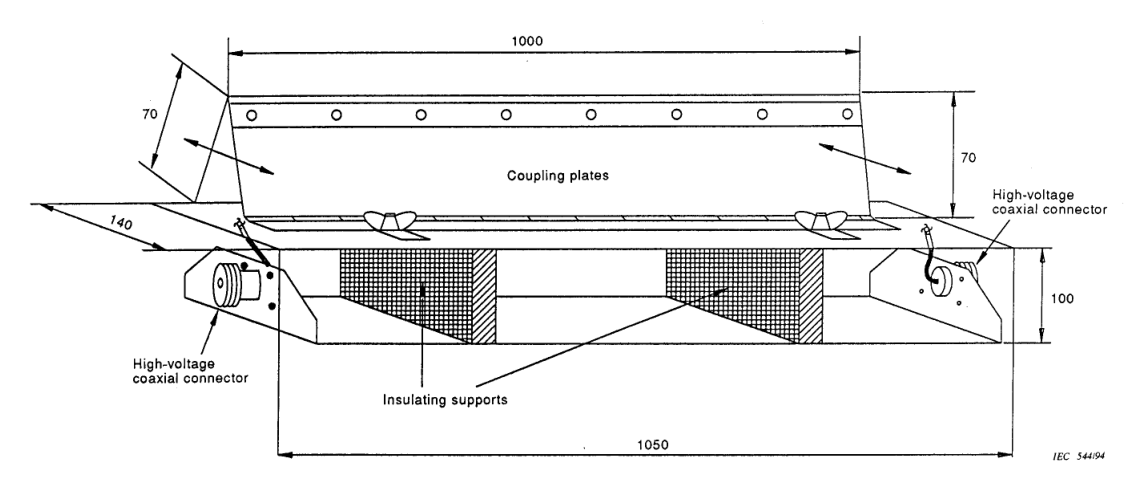
\includegraphics[width=0.8\textwidth]{src/1/figures/iec61000-4-4_clamp.png}
  \caption{IEC 61000-4-4 capacitive coupling clamp}
  \label{fig:iec_4_4_clamp}
\end{figure}

\subsection{IEC 62215 standard}

% Where does this standard applies - scope
The IEC 62215 standard \cite{iec62215} defines a method for measuring the immunity of an integrated circuit to conducted electrical transient disturbances.
This standard specifically targets testing of integrated circuits in operation, and as such is extremely relevant for this document.
In itself, the standard does not define a new test waveform.
It specifies to employ waveforms in ISO 7637-2 \cite{iso7637-2} for automotive devices and IEC 61000-4-4 \cite{iec61000-4-4} or IEC 61000-4-5 for industrial and consumer applications.
It focuses on understanding interactions between a conducted disturbance and performance degradation induced in integrated circuits.
The test method is quite similar to \gls{dpi} defined in IEC 62132-4 \cite{iec62132-4}.
The \gls{dpi} standard focuses on frequency domain immunity, while this standard tests time-domain immunity.

% How is the pulse generated
Disturbances are applied to the \gls{ic} pins via a coupling network.
A typical pin injection setup is given in Fig. \ref{fig:iec62215_setup}.

\begin{figure}[!h]
  \centering
  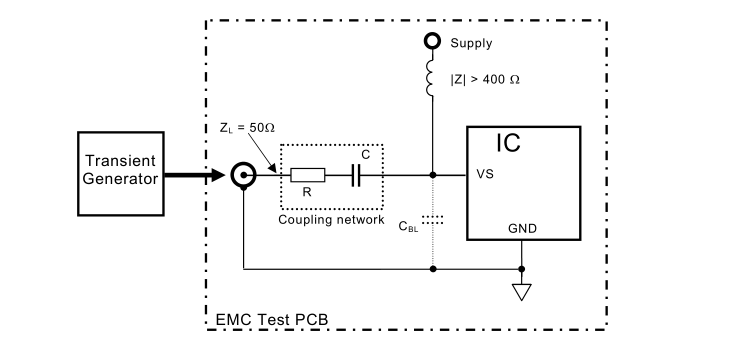
\includegraphics[width=0.9\textwidth]{src/1/figures/iec62215_setup.png}
  \caption{Typical injection setup via a coupling network}
  \label{fig:iec62215_setup}
\end{figure}

% Talk about immunity classes
Beyond test setup and waveforms, the standard defines immunity classes to categorize the behavior of integrated circuits exposed to disturbances during normal operation.
Classes range from A to E, with A describing the most robust devices in terms of functionnality.
In class A\textsubscript{IC}, the \gls{ic} performs within the defined tolerances during and after exposure to disturbance.
In class D\textsubscript{IC}, at least one monitored function of the IC does not perform within the defined tolerances during exposure and does not return to normal operation by itself, requiring an external intervention such as power reset.
In class E\textsubscript{IC}, at least one monitored function does not perform within the defined tolerances after exposure and can not be returned to proper operation.
